\section{Persistence}

\begin{figure}[!htb]
    \centering
    \includegraphics[width=0.8\textwidth]{figures/DB Screenshot users.png}
    \caption{A document showcasing a user, in this case an admin, in the database}
    \label{fig:userDB}
\end{figure}

\begin{figure}[!htb]
    \centering
    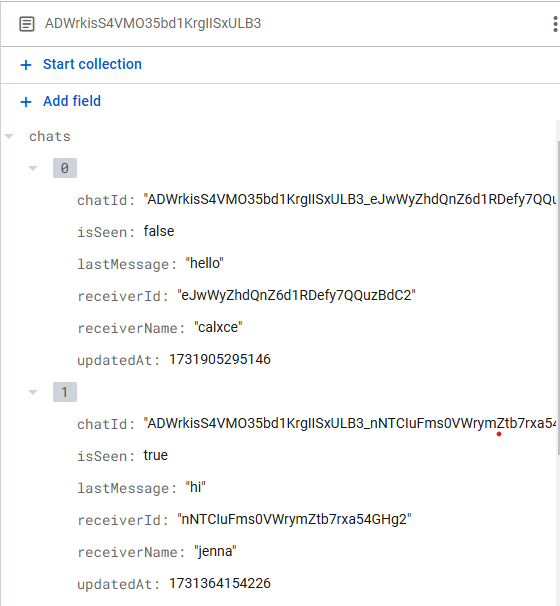
\includegraphics[width=0.8\textwidth]{figures/DB Screenshot userChats.png}
    \caption{A document showcasing a userChat in the database}
    \label{fig:userChatDB}
\end{figure}

\begin{figure}[!htb]
    \centering
    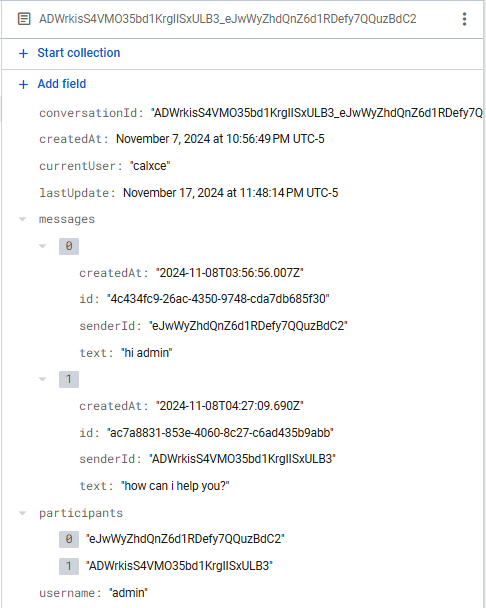
\includegraphics[width=0.8\textwidth]{figures/DB Screenshot conversations.png}
    \caption{A document showcasing a conversation in the database}
    \label{fig:conversationDB}
\end{figure}

\begin{figure}[!htb]
    \centering
    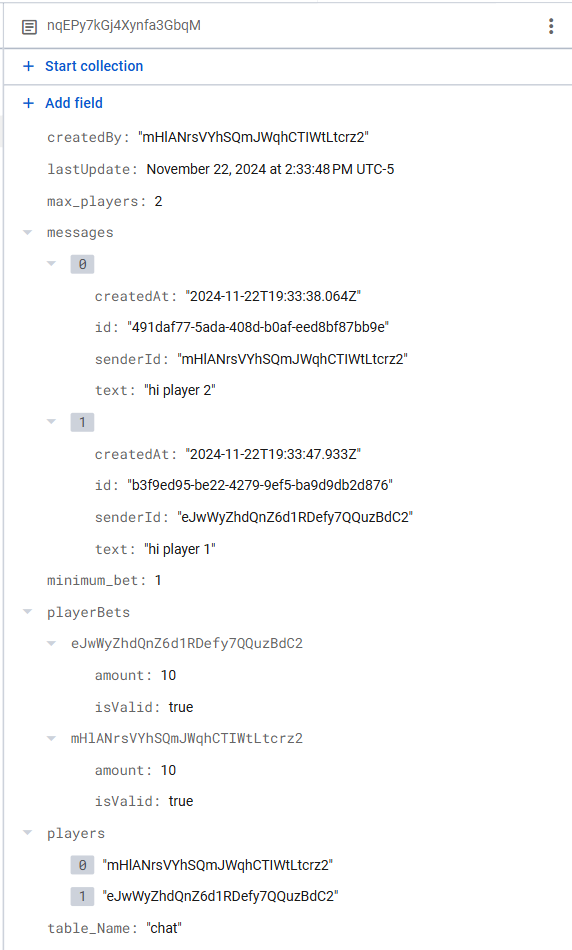
\includegraphics[width=0.7\textwidth]{figures/DB Screenshot table.png}
    \caption{A document showcasing a table in the database}
    \label{fig:tableDB}
\end{figure}

We used Firebase, a NoSQL database to store our persistent data. We created four collections, users, conversations, userChats, and table to store user information, messages among account owners, and table information. The users collection contains fields like email, first name, last name, user ID, username, a list of friends, total wins and losses, their chip balance, and role which can either be an account user or admin. UserChats contains data detailing the most recent updates of a conversation with another user. It includes a chat ID, a Boolean isSeen to indicate whether the message was read, a receiver id, receiver name, the last message sent in the conversation, and a timestamp for last message sent. The conversations collection holds the messages sent between two users. It stores the conversation ID, timestamps for when the conversation was initially created, of the latest update, and a list of participants which stores the two users’ user IDs. There is also a field called messages that is an array of maps. Each map contains fields for the text of a message, the user ID of the sender, a timestamp for when the message was created, and a message ID.

 The table collection stores information about the table as well as the current round being played. It stores the user ID of the host as the creator of the table, the table name, the user IDs of players currently sitting at the table, the table’s minimum bet, max players, and each player’s bet for the round. To indicate a game is in session, the gameStarted Boolean is set to true. It also stores the ID of the current player in the session, each individual’s hand (the suit and rank of the card and its value), the dealer’s hand, and the player’s statuses (if they won the round, busted, or dealer won). Table messages are also stored in this collection in the same format as conversation.

 \clearpage
